\documentclass[a4paper,oneside,12pt]{book}
\usepackage[utf8]{inputenc}
\usepackage[greek,french]{babel}
\usepackage[T1]{fontenc}
\usepackage[utf8]{inputenc}
\usepackage{fvextra}
\usepackage[xetex]{graphicx}
\usepackage{minted}
\usepackage{hyperref}
\usepackage{setspace}%espacement
\usepackage[margin=2.5cm]{geometry}
\usepackage{setspace}
\usepackage{enumerate,lettrine}
\usepackage[babel]{csquotes}
\usepackage[backend=biber, sorting=nyt, style=enc]{biblatex}
\addbibresource{references.bib}
\setlength{\parindent}{1cm}
\onehalfspacing
\hyphenation{}
\hypersetup{}

%%%Mise en page citations pour début de chapitre
\def\changemargin#1#2{\list{}{\rightmargin#2\leftmargin#1}\item[]}
\let\endchangemargin=\endlist 
%paquet pour les annexes
\usepackage{appendix}
\usepackage[acronym,toc]{glossaries}
\makeglossaries
%Pour tourner les images
\usepackage{rotating}
\usepackage{tikz}


\title{Mémoire de M1}
\author{Lily Grumbach}
\date{June 2021}

\begin{document}


\frontmatter

\begin{titlepage}
\begin{center}

\bigskip

\begin{large}
UNIVERSITÉ PARIS, SCIENCES \& LETTRES
\end{large}
%TODO: nom établissement de préparation
\begin{center}\rule{2cm}{0.02cm}\end{center}

\bigskip
\bigskip
\bigskip
\begin{Large}
\textbf{Lily Grumbach}\\
\end{Large}
\begin{normalsize} \textit{licenciée d'histoire}\\
 du Cycle pluridisciplinaire d'études supérieures\\
 de l'Université PSL
\end{normalsize}

\bigskip
\bigskip
\bigskip

\begin{Huge}
\textbf{Revues, santé et territoires}\\
\textbf{en situation coloniale}\\
\end{Huge}
\bigskip
\begin{LARGE}
\textbf{Rapport d'étape}\\
\end{LARGE}

\bigskip
\bigskip
\bigskip
\begin{large}
\end{large}
\vfill

\begin{large}
Mémoire de première année de master\\
\og Humanités numériques et computationnelles \fg{} \\
\bigskip
2021
\end{large}

\end{center}
\end{titlepage}

\thispagestyle{empty}

\cleardoublepage

\section*{Résumé}
\addcontentsline{toc}{chapter}{Résumé}

Ce mémoire s'attache à présenter les méthodes quantitatives et computationnelles pour l'analyse de trois revues majeures de médecine et de santé profondément ancrées dans le développement de l'empire colonial français : les Annales d'hygiène et de médecine coloniales, les Archives de médecine navale et le Bulletin de la Société de Pathologie exotique. 
 
Si les \textit{Periodical studies} se sont développées ces dernières années, les trois sources que nous étudions, connues des historiens n'ont pourtant jusqu'ici jamais été considérés comme objet d'étude à part entière. 
Nous tenterons ici de mettre en lumière les apports des outils numériques pour l'étude comparée de ces trois revues. Nos recherches au cours de cette première année de master ont été essentiellement exploratoires étant donné la nouveauté des outils à maîtriser. Son objectif est donc notamment de mettre en exergue les problématiques et exploitations que nous souhaiterions mettre en place pour notre année prochaine. \\

\medskip

\textbf{Mots-clés:} Médecine ; Santé ; Revues scientifiques ; Histoire ; Géographie ; Humanités numériques

\textbf{Informations bibliographiques:} Lily Grumbach, \textit{Titre du mémoire: sous-titre}, mémoire de master 1 \og Humanités numériques et computationnelles\fg{}, dir. [Anne Rasmussen, Claire Fredj, Carmen Brando], Université Paris, Sciences \& Lettres, 2021.


\section*{Abstract}
\addcontentsline{toc}{chapter}{Abstract}

This dissertation focuses on developing quantitative and computational methods for the analysis of three major medical and health journals deeply rooted in the development of the French colonial empire: the Annales d'hygiène et de médecine coloniales, the Archives de médecine navale, and the Bulletin de la Société de Pathologie exotique. \\
Although periodical studies have developed in recent years, the three sources we are studying, known to historians, have never been considered as objects of study in their own right. We will try to highlight the contributions of digital tools for the comparative study of these three journals. Our research during this first year of the Master's program has been essentially exploratory, given the novelty of the tools to be mastered. Its purpose is therefore to highlight the problems and exploitations that we would like to put in place for our next year. 


\medskip

\textbf{Keywords:} Medicine ; Health ; Sientific Journals ; History ; Geography ; Digital Humanities

\textbf{Bibliographic Information:} Lily Grumbach, \textit{Title: Subtitle}, M.A. thesis \og Digital and computational humanities\fg{}, dir. [Anne Rasmussen, Claire Fredj, Carmen Brando], Université Paris, Sciences \& Lettres, 2021.


\clearpage
\thispagestyle{empty}
\cleardoublepage

\tableofcontents

\cleardoublepage
\cleardoublepage


\vspace*{\stretch{1}}

\begin{flushright}
A Françoise Grumbach
\end{flushright}

\begin{changemargin}{5cm}{0cm} 
\small
Une boîte en carton légèrement effritée, oubliée au fond de la cave. En l'ouvrant, se répandent des articles, lettres, livres, descriptifs de séminaires. \og Tuberculose\fg, \og Inde \fg, \og Afrique \fg, \og Levaditi \fg, \og Pasteur \fg, \og Calmette \fg, ... le nom de Françoise Grumbach traverse ces documents. 
Ils font vivre la mémoire d'une grand-mère jamais rencontrée mais qui a marqué notre famille par son histoire singulière, de la Résistance française en Algérie jusqu'à son laboratoire du service de tuberculose de l'Institut Pasteur. Nous avons, au cours de nos recherches retrouvé certains de ses collègues. Les recherches menées au fil de ce master lui sont adressées. 
\end{changemargin}
\vspace*{\stretch{1}}

\cleardoublepage
\medskip
\medskip
\medskip
\mainmatter
%%%%%%%%%%%%%%%%%%%%%%%%%%% INTRO %%%%%%%%%%%%%%%%%%%%%%%%%%%
\mainmatter
\chapter*{Introduction}

\subsubsection{Revues en situations coloniales}
%% ACCROCHE%% 
Apanage du « Prométhée colonial », la médecine est, avec l’éducation, au cœur des discours de légitimation de la colonisation au nom de la « mission civilisatrice » des États colonisateurs. Or, si les sciences de la nature ont fait l'objet de nombreuses sollicitations par les autorités coloniales pour la \og mise en valeur des colonies\fg, il est nécessaire de restituer les stratégies institutionnelles des réseaux scientifiques à l'aune des bénéfices épistémologiques de l'inscription de leurs recherches dans un cadre colonial\footnote{\cite{bonneuil_savants_1991}}.
Dans cette mesure, en nous interrogeant sur les conditions matérielles, sociales et géographique de ces ces réseaux scientifiques, l'objet revue s'est imposé comme une source riche. Les revues, en tant que \og journaux professionnels \fg \footnote{Jean Delhombre, cité par \cite{tesniere_au_2021}} sont alors des supports majeurs pour saisir l'évolution de champs scientifiques dédiés. 

Ces considérations prennent une envergure particulière dans le cadre des disciplines médicales en situation coloniale. En effet, si les disciplines médicales se sont très tôt munies de revues\footnote{\cite{tesniere_les_2014}}, l’importante distance physique des médecins en situation coloniale, leur confrontation à des milieux pathogènes peu connus et les enjeux politiques dont ils avaient la charge (notamment assurer la santé des européens puis celle des ouvriers et enfin des populations locales) firent des revues médicales un objet clé de la colonisation.  Développées dans l’ensemble des pays colonisateurs, les revues médicales dédiées aux situations coloniales ont permis à la fois de mettre en valeur les avancées de chaque pays dans une optique de compétition mais aussi de permettre une coopération transimpériale sur des thématiques communes, difficilement retenues par des frontières politiques.

%%%%%HISTORIOGRAPHIE%%%%%

\section*{Historiographie}

Tant au regard de l'étude des sciences que de l'histoire des sociétés coloniales, les années 1990 ont marqué un tournant historiographique. En réaction au développement du post-colonialisme dans les universités anglo-saxonnes, divers chercheurs\footnote{Tels que \cite{cooper_tensions_1997}} se sont attachés à « repenser le colonialisme »  en considérant une approche socio-historique du fait colonial ainsi qu'en cherchant à percer les relations complexes entre populations colonisées et coloniales. Ce renouvellement s'est aussi matérialisé dans une  l'étude des interactions entre médecine, empires et gouvernement colonial\footnote{\cite{anderson_where_1998,marks_what_1997,arnold_imperial_1989,harrison_towards_1990}}. Une nouvelle historiographie a notamment été marquée par l'intégration de l’histoire de la médecine coloniale dans l’histoire sociale de la médecine, déplaçant le centre de gravité des métropoles vers les mondes « non européens », les périphéries impériales et les espaces transnationaux. 

En France, ce mouvement a été amorcé au tournant des années 2000 par la publication d'un ensemble de thèses et mémoires interrogeant la construction de savoirs en situation coloniale ou bien l'émergence de spécialités dites "coloniales". \footnote{\cite{sibeud_construction_1999,singaravelou_ecole_1999,blais_les_2000,monnais-rousselot_medecine_1999,bretelle-establet_sante_1999,singaravelou_promethee_2013}}. 
Plus récemment, des chercheurs français tels que Guillaume Lachenal\footnote{\cite{lachenal_medecin_2010}} ont étudié l'enjeu particulier du \og laboratoire colonial \fg et de l'expérimentation. En travaillant sur un archétype de \of laboratoire en plein air \fg qu'a été l'expérience d'Eugène Jamot dans le Haut-Nyong Camerounais dans l'entre-deux guerres, il parvient à « estimer l’effet matériel et symbolique des politiques et des discours médicaux »\footnote{\cite{lachenal_medecin_2010}p.123}, s'inscrivant ainsi dans la continuité des études portées par Stoler et Cooper\footnote{\cite{cooper_tensions_1997}} visant à réévaluer les discours officiels à l'aune des réalités du terrain. Ainsi, entre discours et réalités, le rapport au terrain, au territoire est d'autant plus important que les médecins ont eu un rôle majeur dans la maîtrise des espaces par la maîtrise des maladies.  


A partir de 1880, le développement de nouveaux paradigmes scientifiques (théorie des germes, rôle des parasites) ainsi que l’expansion et la stabilisation des domaines coloniaux et l’institutionnalisation des « sciences coloniales » font de la communication scientifique un enjeu majeur de pouvoir tant dans un cadre de compétition que de coopération entre États. Dès lors, la communication scientifique entre métropole et colonies mais aussi entre les colonies et avec les autres empires coloniaux prend une place de premier ordre. Dans cette mesure, nous nous sommes intéressés à la construction et à la circulation des réseaux de savoirs en une période où les relations scientifiques se structurent autour de congrès internationaux, revues et sociétés savantes dans un contexte d'accélération générale des circulations tant humaines que matérielles et financières.

 %%%REVUES MEDICALES

 \subsubsection*{Appréhender l'objet revue médicale}
Les revues scientifiques sont, à cet égard, une source particulièrement riche d'information. Développées à la fin du XVIIIe et au début du XIXe siècle, l'émergence de la revue résulte du développement du modèle des Sociétés savantes comme lieux de savoir, de socialisation et de positionnement scientifique. Depuis les années 1970, la sociologie des sciences a mis en avant "le rôle des revues dans l'émergence des communautés scientifiques et dans la formation des disciplines "\footnote{\cite{duclert_les_2002},p.239}. Leur émergence a aussi été conditionnée par l'accélération des échanges et l'abaissement des prix d'envois. 
Leur histoire est donc avant toute chose celle d'une \og mécanisation et marchandisation du régime épistolaire par le développement de l’imprimerie et des maisons d'édition\fg \footnote{\cite{guedon_lhistoire_2017,tesniere_au_2021}}. Remplaçant les correspondances interpersonnelles, l'objet revue en contribuant à la constitution de réseaux scientifiques plus larges contribue ainsi non seulement à créer des normes linguistiques et argumentatives d'un champ mais aussi, par leur démultiplication numérique depuis 1880, à accroître les spécialisations. L'industrialisation de l’imprimerie et la modernisation des transports au XIXe siècle bouleversent alors les conditions de constitution et de transmission des connaissances. Un des intérêt de l'analyse de la production éditoriale pour nous est donc de saisir « l’intrication complexe de la médecine généraliste et des spécialités avec les préoccupations de santé publique et de formation professionnelle »\footnote{\cite{tesniere_les_2014}}. 


\subsubsection{Quelle discipline pour la médecine en situation coloniale ? }
Définir ce que recouvrent les dénominations de médecine "coloniales", "tropicales", "exotiques", "navale", peut être appréhendé au travers une étude rapprochée des revues qui se présentent comme relevant de ces "spécialisations" en étudiant précisément comment elles se différencient par les thématiques abordées mais aussi par les références employées et les acteurs qui y prennent part. Plusieurs historiens ont tenté de différencier ces dénominations de spécialités médicales : en fonction de la formation des acteurs qui s'en revendiquent\footnote{\cite{cook_rise_2014,braesco_former_2017,osborne_emergence_2014}}, au regard des réseaux d'acteurs formés en \og Communauté épistémique \fg\footnote{\cite{haas_introduction_nodate,packard_networks_2012}}, par les discours et utilisations politiques de cette médecine \footnote{\cite{marks_what_1997}} ou en menant une étude sur un terrain précis\footnote{\cite{anderson_colonial_2006,}}.

La thèse de Marie-Albane de Suremain sur \textit{L'Afrique des revues}\footnote{\cite{suremain_de_afrique_2001}} fait office d'exemple pour notre approche en tant qu'elle parvient à interroger, à partir des revues de sciences sociales, l'évolution des acteurs et des structures produisant des savoirs estampillés comme "coloniaux". Cette démarche fait particulièrement écho à ce que nous souhaitons engager pour ce mémoire en tant qu'exemple d'une recherche liant thématiques, espaces et acteurs engagés dans la production de savoirs en situation coloniale, démontrant, au fil du premier vingtième siècle l'institutionnalisation de la production des sciences sociales dites "coloniales". Si cette étude a été menée sur les revues de sciences humaines et sociales, il n'en existe pas à notre connaissance sur les revues médicales. 

L'étude des revues et plus particulièrement des revues médicales est un lieu commun en histoire des sciences. Mais l'étude plus précise de l'histoire de leur édition reste relativement récente. En effet, l'intérêt des historiens pour la revue scientifique a longtemps été (et est toujours dans une large mesure) au niveau des contributeurs de revues scientifiques\footnote{\cite{csiszar_scientific_2018}} tandis que Valérie Tesniere propose une lecture "terre à terre" de la revue. Suivant les recherches en histoire du livre et de l'édition \footnote{\cite{mollier_argent_1988} et l'Histoire de l'édition française de Roger Chartier et Henri-Jean Martin.}. L'existence de sociétés de recherche dédiées aux questions des revues telles que la  \textit{Research Society for American Periodicals} et la \textit{European Society for Periodical Research} attestent de la vivacité de ce champ de recherche qui s'est trouvé entre autres bouleversé par la numérisation massive des revues. Les démarches d'ouverture des bibliothèques et archives en ligne ont alors permis et accompagné le développement de nouvelles heuristiques grâce à des méthodes de codage et d'encodage des revues que nous envisageons dans le cadre du master humanités numériques de l'université Paris Sciences et Lettres. 






%%%PROBLEMATIQUE%%%%%

\subsection*{}

%%%%%%PROBLEMATIQUE %%%%%%%%%%
Nous retenons ainsi de cette présentation des termes du sujet la possibilité, tant technique qu'épistémologique, de mettre en lumière, grâce aux méthodes apportées par les humanités numériques et au travers de l'objet d'étude particulier qu'est la revue, de nouvelles manières de comprendre le triptyque entre un réseau d'acteurs, des enjeux de santé et des territoires d'exercice particuliers que sont les territoires coloniaux. A cet égard, nous avons choisit de travailler sur trois revues qui entretiennent des liens particuliers de par le partage de leurs acteurs, de leurs thématiques et, à priori, de leur terrain. Les Annales d'hygiène et de médecine coloniales (qui deviennent en 1919 les Annales de médecine et de pharmacie coloniales), les Archives de médecine navale (qui deviennent en 1914 les Archives de médecine et de pharmacie navales) et le Bulletin de la Société de pathologie exotique.

Bien connu des chercheurs s’intéressant à ces problématiques, ces trois revues n'ont jamais fait l'objet d'une étude approfondie.  Pour cette année, nous avons souhaité mettre en place un ensemble de matériaux et de méthodes qui nous permettront de mettre en oeuvre comme il se doit nos recherches l'année prochaine et de répondre aux questions de recherche que nous avons évoqué jusqu'ici.



%%%DESCRIPTION DES SOURCES%%%
\subsection*{Pistes proposées pour l'étude de nos revues}

Les humanités numériques offrent à notre avis une nouvelle heuristique pour aborder des sources aussi denses que les revues. Notre objectif est ici de rendre compte des explorations des sources que nous avons mis en place au fil de cette année particulière et riche en découvertes.
Cet enivrement des nouvelles méthodes d'analyse nous a par moment poussé à envisager de (trop) nombreuses pistes de recherche qui n'ont pas toujours pu aboutir cette année en raison des (aussi trop) nombreux engagement.

nous avons souhaité explorer quelques pistes pouvant répondre à nos multiples interrogations afin de nous procurer les matériaux et méthodes pour une analyse approfondie au cours de l'année prochaine.












%%%%%%%%%%%%%%%%%%%%%%%%%%% CHAPITRE 1 %%%%%%%%%%%%%%%%%%%%%%%%%%%
\chapter{Trois revues de santé en situation coloniale}

\section*{Du papier à l'écran, un autre goût des archives}

%%%%%% HN HN HN HN HN HN %%%%%%%

Internet s’est aujourd’hui imposé comme la première source d’information. Ainsi, notre découverte des trois revues traitées s'est avant toute chose faite en ligne. Des bibliothèques universitaires
\footnote{https://www.biusante.parisdescartes.fr/histoire/medica, consulté le 20/05/2021} à Internet archive\footnote{https://archive.org/, consulté le 20/05/2021}, nos revues peuvent être caractérisées par une très grande accessibilité numérique. 
Leur numérisation est le fruit du travail engagé dès 2005 par la Bibliothèque interuniversitaire de médecine(BIUS)\footnote{Nous souhaitons à cet égard remercier M.Jean-François Vincent et Mme Solène Coutagne, chefs du service historique de la Bibliothèque interuniversitaire de santé, d'avoir répondu à nos questions et de nous avoir fait parvenir les cahiers des charges de chaque revue que nous étudions afin de saisir comment ce projet de numérisation précoce a été conçu ainsi que comment ces choix initiaux ont déterminé la lecture que nous pouvons en avoir aujourd'hui.}. 

Dans le cadre français, les Annales d’hygiène et de médecine coloniale (AHMC), les Archives de médecine navale (AMN) et le Bulletin de la société de Pathologie exotique (BSPE) ont tenu ce rôle d’organe de communication et de rayonnement des avancées françaises mais un trait de caractère les différencie toutefois grandement. Tandis que les AHMC et AMN dépendent d'un corps de métier définit par et sous l'égide d'administrations gouvernementales, le Bulletin dépend pour sa part d'une société savante reposant d'une part sur la notoriété de ses fondateurs et de ses membres honoraires et d'autre part sur les scientifiques présents sur le terrain. Or toute trois partagent des thématiques et acteurs communs dont nous avons cherché à retracer la généalogie.

En portant notre regard sur les revues, nous cherchons à déceler non pas tant le cheminement de leurs recherches mais bien ce que les diverses institutions ont souhaité \og donner à voir \fg. Dans cette partie nous cherchons donc à mettre en exergue les particularités et point communs de chacune des revues avant d'en déployer les inter-relations. Nous verrons dans un premier temps ce qui lie les acteurs et thématiques des Archives de médecine navale et les Annales d'Hygiène et de médecine coloniales avant de les lier à la Société de Pathologie exotique.\footnote{cf la Figure 3 en annexe} 

%%%%%%%%%%%%%%%%%Deux revues institutionnelles%%%%%%%%%%%%%%%%%%%%%%
\section{Deux revues institutionnelles à la généalogie commune : les Archives de médecine navale et les Annales d'Hygiène et de médecine coloniales}

Parmi les trois revues que nous étudions, les Archives de médecine navale et les Annales d'Hygiène et de médecine coloniale ont la particularité de dépendre de ministères. D’une part le ministère des Colonies et le Corps de santé des Troupes coloniales. D’autre part, celui de la Marine et le corps de santé navale. 
Ces deux ministères sont le produit d'une scission en 1890 du Ministère de la Marine et des Colonies, témoignant d'une démarche d'autonomisation du champ colonial par rapport à la navale dont il dépendait jusqu'alors. Dans ce cadre, les deux revues institutionnelles traitées ont un triple objectif : administratif, corporatiste et scientifique. Les liens entre les deux corps restent néanmoins majeurs. 


En effet, l'accès au Corps du Service de santé des troupes coloniales est avant tout présenté comme une forme de "spécialité" des médecins sortant du corps de la navale. Pour intégrer ce corps, il est nécessaire de passer d'abord par une classe préparatoire au concours de l'Ecole militaire de Santé navale pour ensuite intégrer l'Ecole de santé navale de Bordeaux (créée en 1890). La création en 1905 de l'Ecole d'Application du Service de Santé des Troupes Coloniales à Marseille (Le Pharo) fixe le cadre d'un domaine scientifique\footnote{Pour une analyse détaillée du fonctionnement de l'Ecole du Pharo, voir \cite{braesco_former_2017}}. Selon Camille Braesco, la médecine tropicale devient coloniale dans la mesure où elle a trait à des territoires coloniaux. Mais elle ne se résume pas pour autant à la médecine tropicale puisque la formation même des acteurs met avant tout en exergue la capacité d'adaptation de chacun à des situations très variées et ne repose donc pas tant sur l'acquisition de connaissances théoriques particulièrement plus poussées sur les maladies tropicales ni sur les particularités locales des pays colonisés.



\subsection{Les Archives de médecine navale}
Les Archives de médecine navale sont fondées en 1864 par le ministre de la Marine et des Colonies Chasseloup-Laubat et dirigé par Leroy de Méricourt. 180 ans après la création du Service de Santé navale par Signelay et treize années après la première Conférence sanitaire internationale, la création des Archives de médecine navale est le fruit de plusieurs décennies de tentative de création d'un journal relatif au Service de Santé navale\footnote{Voir Archives de médecine navale 1864, n° 01. - Paris : J.-B. Baillière, p.5.}. Les AMN ont d'abord été éditées chez J.B. Baillière (1864-1881), "libraires de l'académie impériale de médecine" jusqu'à l'établissement de la IIIe République, avant d'être publié chez Octave Doin jusqu'à la fin de la Première Guerre mondiale qui la verra être reprise par l'Imprimerie nationale. Cette évolution témoigne de l'évolution du marché éditorial scientifique et des choix de . En effet, les deux changements de maison d'édition sont marquées, dans un premier temps par la progressive perte de vitesse des éditions Baillière dans le domaine de l'édition de revues (notamment dépassé par les éditions Masson\footnote{\cite{tesniere_au_2021}}, qui gèrent depuis 1908 le Bulletin de la Société de Pathologie exotique ) puis par le changement de direction de la maison d'édition Doin et les difficultés financières suite à la Première guerre mondiale\footnote{Cette partie gagnerait à être approfondie par la consultation des archives de chaque maison d'édition.}. 

A partir de la création de Corps de santé des troupes coloniales, les médecins de la marine ont été majoritairement cantonnés aux ports métropolitains, comme en atteste la Reconnaissance d'entités nommées que nous avons menée sur cette revue puis cartographié à l'aide de QGIS (cf Annexe 3)

\subsection{Les Annales d'hygiène et de médecine coloniale}

\begin{changemargin}{5cm}{0cm} 
« La pathologie exotique offre un vaste champ d’études où il y a encore beaucoup à glaner. Notre domaine colonial s’est tellement étendu dans ces dernières années que presque tout est à faire, au point de vue de la géographie médicale. »\footnote{Alexandre Kermorgant, “Introduction”, Annales d’Hygiène et de médecine coloniales, vol.1,n°1, 1898, p.6.}
\end{changemargin}

En posant \og la pathologie exotique \fg et la \og géographique médicale \fg comme principaux domaines d'étude affilié au corps de santé des troupes coloniales, Alexandre Kermorgant, fondateur de la revue et futur membre fondateur de la Société de pathologie exotique (SPE), d'une part s'inscrit dans la continuité des Archives de médecine navale qui débutait déjà chaque numéro de sa revue par un article de géographie médicale. D'autre part il insiste, par la notion de \og pathologie exotique \fg à l'acception réifiante de l'altérité, qu'elle soit géographique ou pathologique. Pourtant, ce fort déterminisme entre lieux, environnements et effets sur la santé alimentés par les pratiques de topographies médicales a été remis en question à la fin du XIXe et début du XXe siècle par la théorie des germes et la découverte des agents pathogènes. Ainsi, si les "Contributions à la géographie médicale" ouvrent chaque numéro de la revue jusqu'à 1914, cette catégorie disparaît par la suite. La disparition de cette catégorie peut aussi s'expliquer par un changement générationnel des contributeurs à la revue à partir de l'après Seconde guerre mondiale, ainsi que la création de la Société de pathologie exotique en 1908 qui devient la principale référence des Annales comme en témoigne, à partir de 1924, la part importante des références au bulletin de la Société au point de constituer, à partir de 1927 presque une rubrique entière rendant compte des principaux apports des séances de la SPE. 

Cette relation des médecins du corps de santé coloniale avec la microbiologie est notamment marquée par le rôle de ces derniers dans la fondation des Instituts Pasteur d'outre-mer\footnote{Calmette (Saigon), Yersin(Nha-Trang), Simond (Karachi), Roubaud (Brazzaville), Mathis (Hanoi), Girard et Robic (Tananarive), Laigret (Dakar).} ainsi que l'importance de la part de leurs contributions au Bulletin de la Société de pathologie exotique. En effet, le rapport intime des médecins coloniaux au terrain permet à ces derniers de prendre pleinement part à la vie de la société par l'envoi d'échantillons et la rédaction d'articles\footnote{Nous avons effectué une liste à visée prosopographique de l'ensemble des médecins des troupes coloniales membres de la Société de pathologie exotique mais n'avons pas eu le temps cette année de l'exploiter convenablement pour une analyse à présenter dans ce premier rendu.}. 

\section{Le Bulletin de la Société de Pathologie exotique}

\begin{changemargin}{5cm}{0cm} 
« ARTICLE PREMIER. – La Société de pathologie exotique a pour but l’étude des maladies exotiques de l’homme et des animaux ; celle de l’hygiène coloniale et de l’hygiène navale et des mesures sanitaires destinées à empêcher l’extension des épidémies et des épizooties d’origine exotique. »
\end{changemargin}
\begin{flushright}
\small
Statuts de la Société de Pathologie exotique, 1907
\end{flushright}

Créée en 1907, la Société de pathologie exotique (SPE) se définit par un rapport à l’exotique. Tant géographique que pathologique, l’exotique exprime ici une mise à distance d’objets d’étude, accessibles uniquement par le voyage, ainsi qu’une extériorisation de l’Autre en le rapportant à des manifestations extérieures relevant de pathologies supposées inconnues. En dressant l’endiguement des « épidémies et épizooties d’origine exotique » comme objectif ainsi qu’en se revendiquant de l’hygiène coloniale et navale, les fondateurs de la société mettent de facto leurs travaux dans le cadre de l’intérêt des autorités politiques françaises mais aussi européennes. 
De par la notoriété de ses membres français comme étrangers, sa proximité au pouvoir politique et la puissante maison d’édition Masson \& Cie, la Société de pathologie exotique a fait de son Bulletin (BSPE) un support majeur de communication scientifique parmi les nombreux nouveaux titres de périodiques caractérisant la « Belle Époque des revues » 2 . Toujours publiée aujourd’hui sous le même nom et par la même maison d’édition\footnote{Malgré le fusionnement en 2005 de Masson avec Elsevier.}, le BSPE a traversé le XXe siècle tandis que la majorité des titres créés pendant cette période n'ont pas survécu à l'arrêt de la Première guerre mondiale \footnote{\cite{tesniere_les_2014}}/ 

L’objectif premier du BSPE est de donner à lire les activités de la SPE. Aux réunions mensuelles correspondent un numéro du Bulletin, la société rend compte de ses correspondances et échanges avec diverses personnalités ou lecteurs ou encore la retranscription de discussions à l’issue d’une communication. Par ailleurs, comme pour toute société savante, par un processus de sélection tant des membres que des communications et mémoires pouvant être faite au cours des séances de la SPE puis être imprimées. A cet égard, il serait nécessaire de se pencher sur les archives même de la SPE auquel nous n’avons pas eu accès pour raison sanitaire15. Ces dernières devraient nous renseigner sur les discussions internes à la Société pour en éclairer finement le fonctionnement interne et le comparer avec ce qui est transcrit dans la revue.
De plus, le capital symbolique de Laveran, des autres membres fondateurs et de l’inscription de la société sous l’égide de l’Institut Pasteur permettent à la SPE d’avoir l’oreille du gouvernement français en métropole comme aux colonies16. Cette position est d’autant plus renforcée par la création dès 1913 de commission de travail s’adressant directement aux pouvoirs publics : opium, maladie du sommeil, paludisme, fièvre jaune font alors l’objet de recherches spécifiques, attribuées à une équipe de membres de la Société chargée de rendre compte aux autorités de leurs recommandations.
Le Bulletin n’est en effet qu’une traduction lissée des activités d’une société éclatée à travers le monde dont les séances ne donnent à voir que les résultats d’un échantillon d’expériences, ne rendant que partiellement compte de l’élaboration des savoirs. Excès de zèle, exagération auto-promotionnelle ou réalité, les présidents successifs de la SPE ont rappelé presque chaque année dans leur allocution à la Société le nombre important de communications qui leur était envoyé supposant un triage important. Il est alors possible, en considérant ces brèches de reconstituer une archéologie des savoirs en œuvre. Elles donnent aussi à voir les différents degrés d’implication des membres de la société savante et d’établir une cartographie professionnelle et géographique de la vie de la revue.



\section{Provincialiser l’Europe?}

Si les trois revues que nous étudions sont éditées en Métropole avant d'être envoyées à travers le monde, il nous semble qu'elles participent à une forme de provincicalisation de l'Europe. En effet, la répartition des médecins de par le monde et la création de laboratoires, d'Instituts Pasteur, et d'Ecole de médecine dans les colonies par des médecins issus notamment des troupes coloniales attestent d'une progressive décentralisation de la production des savoirs. 

Ainsi par exemple, au lendemain de la Grande Guerre, le BSPE rend aussi compte des séances de sociétés devenues « filiales » de la Société de pathologie exotique ; à savoir la Société médico- chirurgicale de l'Ouest africain (SMOA, de 1922 à 1940) et la Société des sciences médicales de Madagascar (SSMM, de 1928 à 1940). Toutes deux liées à l’Institut Pasteur et à l’école de médecine de la ville où elles sont établies, leur fondation par des médecins des troupes coloniales remonte respectivement à 1919 à Dakar et 1909 à Antananarivo. Leur rattachement à la SPE permet alors de gagner grandement en visibilité via le BSPE. Preuve en est qu’aujourd’hui le Bulletin de la SSMM, publié jusqu’à 1928, par exemple n’a pas été numérisé par la BIUS et n’a donc pas le même statut. Du côté de la SPE, l’intérêt d’une filiale permet de rendre compte de son rayonnement en bâtissant à son tour son propre petit empire.


%%%%%%%%%%%%%%%%%%%%%%%%%%% CHAPITRE 2 %%%%%%%%%%%%%%%%%%%%%%%%%%%
\chapter{Réseaux et territoires : une approche par les Humanités numériques}

\subsection{Constituer nos bases de données }

L'accès à nos trois revues sur le site Medica de la Bibliothèque interuniversitaire de médecine a grandement facilité notre tâche de structuration des données des revues toute en la compliquant. En effet, le recours aux regex n'a pas été toujours probant étant donné les différentes indications données par les équipes de la BIUS aux entreprises tierces qui se sont occupées de la numérisation de leurs revues. Nous n'avons pas entièrement terminé de les retraiter car il faudrait encore passer en revue l'intégralité des 50 000 articles qui composent les trois revues sur les quarante années étudiées. Nous avons toutefois pour ce rendu souhaité mettre en avant les quelques avancées que nous avons pu réaliser en outre des nombreuses lectures que nous avons faites et qui ne transparaissent malheureusement pas dans ce mémoire.


\section{Cartographier une revue : rendre compte des logiques spatiales de la science}

L'ensemble des documents et scripts de cette partie se trouvent dans notre repository : https://github.com/LilyG98/Memoire-M1 


La géographie a joué un rôle primordial pour la définition des territoires relevant du pouvoir métropolitain tant d’un point de vue ethnologique que pathologique. Via la géographie médicale, le développement de médecines dites « tropicales », « coloniales », « navales », « exotiques », les a fait dialoguer autour d’un même objet d’étude relevant de l’altérité. La géographie médicale alimente alors une « géographie imaginaire » 5 . Pourtant, le développement de nouveaux paradigmes scientifiques, tels que la théorie des germes et le rôle des parasites dans la transmission de certaines maladies, détourne à plusieurs égards l’importance donnée à la topographie et au climat comme unique étiologie.

Nous avons souhaité considérer la répartition géographique des contributions à nos deux revues afin d’en saisir les territoires d’intérêt. En effet, la publication dans une revue officielle de mémoires originaux et de rapports effectués à l’administration nous renseigne sur ce que les autorités ministérielles estimaient comme pertinent pour la gouvernance des territoires.

Une des majeurs avancées de notre année a donc été de mettre en place une méthode et de collecter les données permettant de cartographier l'ensemble des contributions à nos revues. Cette dernière est le résultat de deux démarches complémentaires. La première est la reconnaissance d'entités nommées que nous avons adapté à notre corpus. La seconde a été la désambiguïsation des entités géographiques repérérés par notre pipeline pour les faire correspondre aux coordonnées géographiques. Cette démarche, a nécessité le recours à deux bases de données à partir desquelles nous avons créé une pipeline dédiée à nos archives : GeoPolHist\footnote{Béatrice Dedinger, \& Paul Girard. (2021). GeoPolHist dataset (Version 202103) [Data set]. Zenodo. http://doi.org/10.5281/zenodo.4600809, consulté le 3 juin 2021} ainsi que l'assistance de recherche géographique des Archives nationales d'Outre-mer \footnote{http://anom.archivesnationales.culture.gouv.fr/geo.php?ir=, consulté le 3 juin 2021}. 


\subsection{Récupération des entités nommées par article}
Dans le cadre du master Humanités numériques, nous avons souhaité proposer un rendu tirant aussi parti de l’enseignement de Traitement automatique de la langue proposé par M. Thierry Poibeau. Ainsi, pour cartographier nos deux revues de 1898 à 1908, nous avons procédé à une reconnaissance d’entités nommées. Cette démarche nous a entre autres permis d’extraire de 1198 titres d’article deux types d’entités nommées aisément cartographiables: les Geopolitical Entities (GPE) et Location (LOC). Les GPE correspondent à l’ensemble des noms de lieux dépendant d’une entité apparentée à une administration (pays, région, province, ville, village etc.). Les LOC désignent pour leur part les entités nommées «purement» géographiques, n’étant pas par le résultat d’une intervention humaine (cours d’eau, montagne, mer, etc.).

En raison de problèmes techniques nous ayant fait perdre la quasi-totalité de nos annotations manuelles sur Doccano, nous avons eu recours au premier de notre 5-fold cross validation set pour entraîner un NLP et l’appliquer à nos sources7. Au total, 559 entités GPE et LOC ont été reconnues par notre NLP parmi lesquelles nous avons décompté 225 lieux différents. Néanmoins, n’ayant pu entraîner totalement notre NLP, nous avons donc eu quelques faux positifs parmi cette liste :

Si certains font référence à des notions scientifiques (Caldwelle-Luc, Danaïde, Surra, Phlégéton), d’autres sont en fait des épithètes liées à des entités GPE ou LOC. Par exemple : « Annamite » se référant à l’Annam, « Bambaras » à la région située entre l’actuel Mail, le Sénégal et le Burkina Faso. D’autres enfin sont le résultat d’une séparation des tokens d’une même EN comme « Nord » qui se trouve être en fait issu de « Cochinchine du Nord » ce qui n’est donc pas totalement incorrect mais tout de même faux au regard des attentes d’une démarche de reconnaissance d’entités nommées.
L’exploration de nos entités nommées GPE nous ont confirmé la nécessité d’avoir un fond de carte permettant de rendre compte de la situation politique de chacune d’entre elles au cours de la période que nous étudions.

\subsection{Le monde au début du XXe siècle}

./data/1-QGIS\_GPH\_HistNatBound.ipynb

Un enjeu principal de notre démarche fut la constitution d’une carte du monde reflétant les frontières d’époque, notamment entre États souverains et territoires dépendants. Pour cela, nous avons eu recours à deux bases de données dont nous avons fait correspondre les entités pour obtenir le fond de carte de notre projet (cf Annexe 2). Nous avons ainsi eu recours aux données de deux projets accessibles librement en ligne.
Le premier est « Historic National Boundaries »de l’Université de Minnesota, disponible sur ArcGIS que nous avons téléchargé en format GeoJSON grâce au SQL d’ArcGIS online. Cette base nous a permis d’avoir les shapes des entités géopolitiques. Le second est les données historiques fournies par le projet GeoPolHist du Medialab porté par Paul Girard 9 . Très complète, cette base de données permet de multiples exploitations grâce au travail de systématisation des données de 1815 à nos jours. Cette base nous a permis de saisir le statut précis des territoires étudiés à la date de 1914.

\textbf{Limites : imprécisions et illusions}

Si ces deux bases de données sont en anglais, elles diffèrent par leur degré de précision. Au regard de notre volonté de cartographier les données, nous avons priorisé les données de l’université de Minnesota au détriment de la précision des données du Médialab. Ainsi par exemple, il n’existe dans la base de données ArcGIS qu’une seule shape pour l’ensemble de l’Algérie, le Haut-Sénégal, le Soudan français et le Burkina Faso alors même que leurs statuts de dépendance à la France n’était pas identique sur toute la période que nous étudions.

Enfin, il nous semble que notre carte est téléologique à plusieurs égards. Premièrement, le fond de carte, trouvé sur ArcGIS, date de 1914 tandis que nos entités débutent en 1898. Deuxièmement, la carte donne l’illusion d’une maîtrise continue du territoire tandis qu’il est nécessaire de considérer les empires comme une "collection éparse de territoires de tailles variables"10 sur laquelle le pouvoir est exercé de manière discontinue.

Comme mentionné précédemment, le principal enjeu de la constituions de cette carte fut la désambiguïsation des noms d’entités géopolitiques et des noms de lieux géographiques.
Pour cela, nous avons eu recours à trois bases de données que nous avons enrichies mutuellement. La raison pour ce recours multiple est que deux de ces bases de données étaient déjà affiliées à des coordonnées géographiques tandis que la troisième nous servait de complément pour les noms de lieux n’apparaissant pas dans les précédentes listes.


%%%%RETOURS CRITIQUES%%%%
\subsection{Retour critique sur notre démarche et projection pour l'an prochain}

Il nous importe de même de mettre cette carte en perspective avec les problématiques relatives à l’appropriation coloniale de l’espace au travers de la construction des savoirs géographiques et des pratiques spatiales. En effet, en aillant recours à une représentation à l’échelle mondiale et datant de 1914, non seulement nous nous conformons à une vision téléologique des appropriations coloniales mais participons de même à supposer que les puissances coloniales avaient un pouvoir continu alors même que certaines régions, comme le Sahara\footnote{Cette région a notamment fait l'objet d'une étude approfondie par Hélène Blais dans \cite{blais_territoires_2020}}, n’étaient que très peu maîtrisées. Cette différenciation, primordiale entre représentation de la domination de l'espace par les savoirs coloniaux et l'espace de la domination en pratique n’a pas pu être développé dans ce premier rendu et nous considérerons pour l’année prochaine une manière d’en rendre mieux compte.


A plus long terme, l’objectif est en effet de nous munir de bases de données et de fonds de cartes exploitables pour notre rendu final de mémoire en M2. En effet, nous souhaitons pour l’an prochain cartographier l’ensemble des contributions aux trois revues que nous étudions et de détailler plus encore le cadre dans lequel ces territoires sont évoqués : compte rendu d’expédition, géographie médicale, clinique, rapports sur d’autres empires etc.). L’idée étant aussi de coupler ces recherches avec du topic modelling sur l’ensemble de notre période (1898- 1940) pour saisir plus précisément le jeu des échelles qui transparaissent dans notre revue, allant du micro au macroscopique, cherchant tantôt dans l’environnement, tantôt dans les cellules, les conditions d’apparition, de développement de certaines pathologies et les moyens pour les endiguer.




%%%%%%%%%%%%%%%%%%%%%%%%%%% CHAPITRE 3 %%%%%%%%%%%%%%%%%%%%%%%%%%%
\input{CHAP3-Adévelopper.tex}

%%%%%%%%%%%%%%%%%%%%%%%%%%% BIBLIO %%%%%%%%%%%%%%%%%%%%%%%%%%%
\printbibliography

%%%%%%%%%%%%%%%%%%%%%%%%%%% ANNEXES %%%%%%%%%%%%%%%%%%%%%%%%%%%

\appendix
\renewcommand{\appendixpagename}{Annexes}
\appendixpage

\begin{figure}
    \centering
    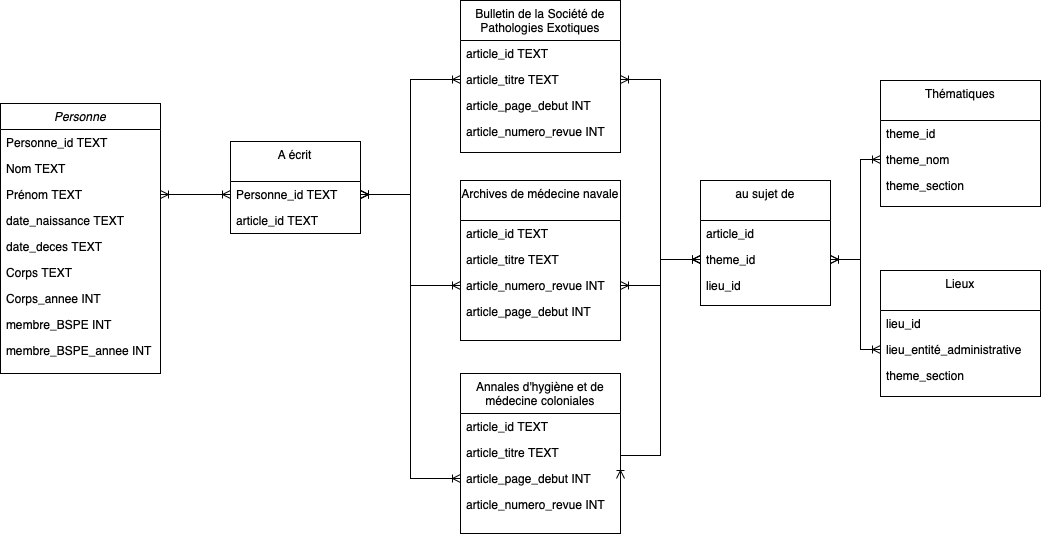
\includegraphics[width=15cm]{./images/Schema-BDD-memoire}
    \caption{Schéma de la base de données relationnelle élaborée avec M. Jolivet}
    \label{Schema-BDD-memoire}
\end{figure}


\begin{figure}
    \centering
    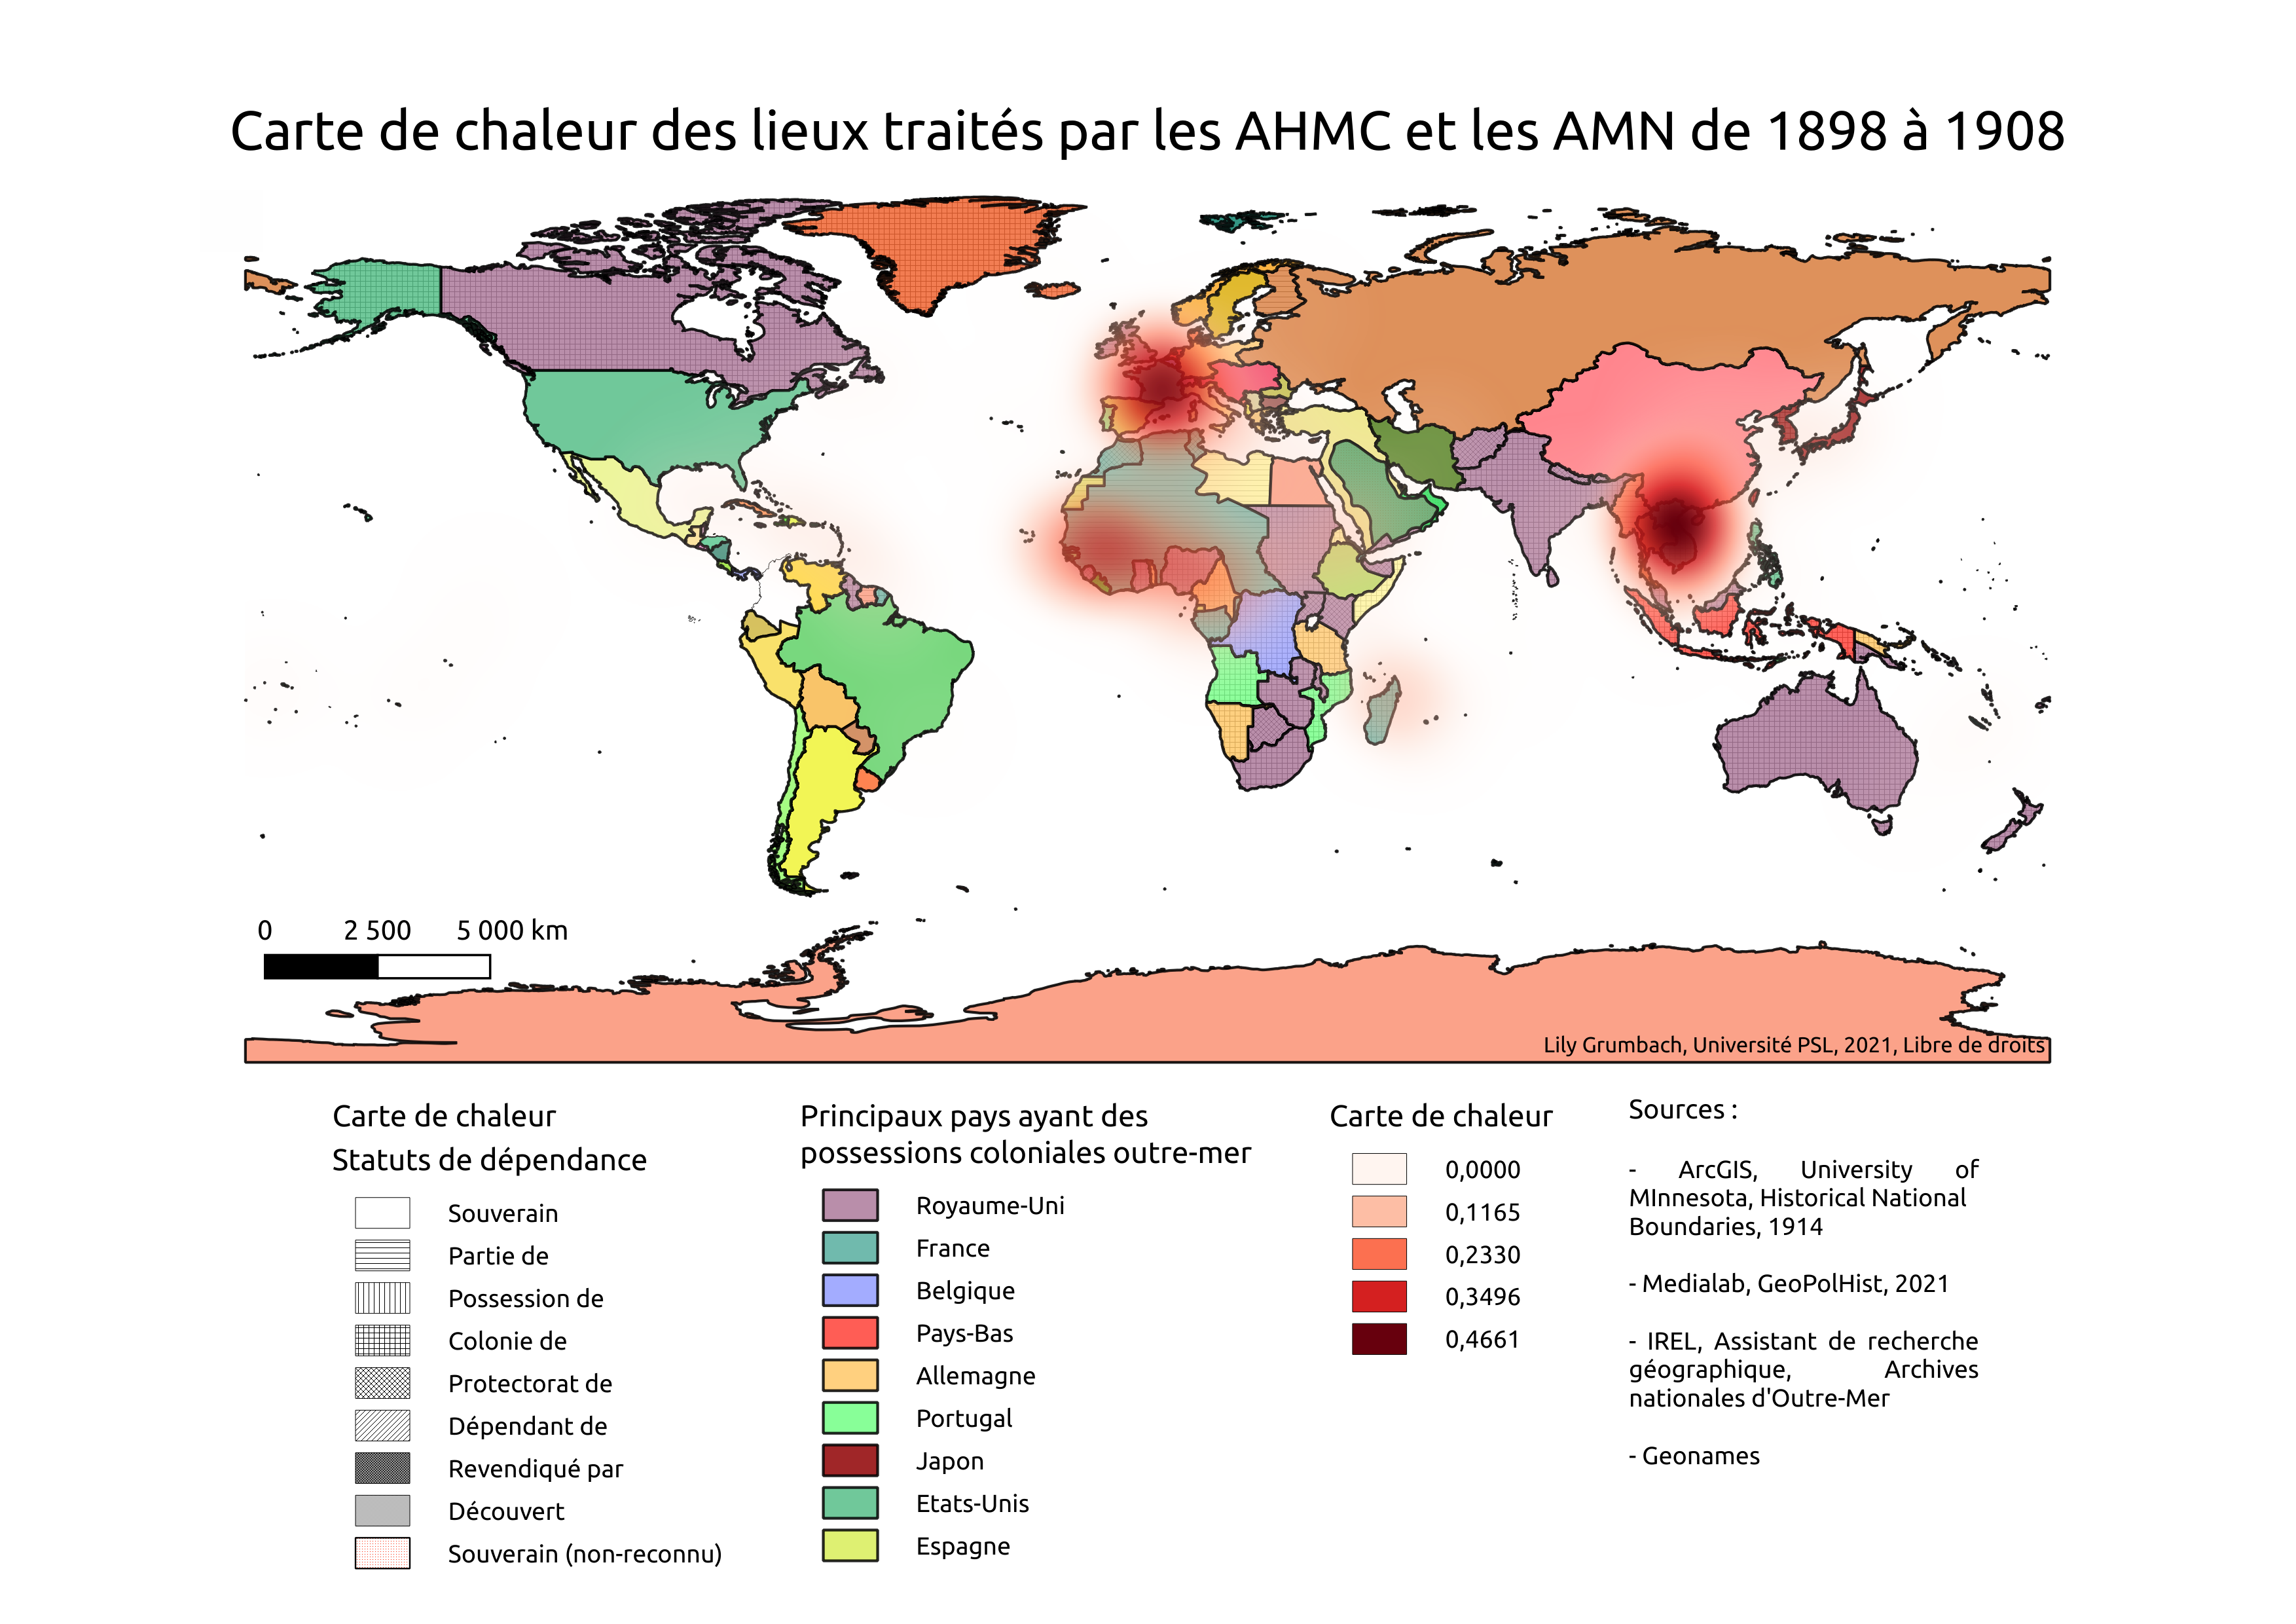
\includegraphics[width=15cm]{./images/Carte_chaleur_AHMC-AMN}
    \caption{Carte de chaleur}
    \label{Schema-BDD-memoire}
\end{figure}



\begin{figure}
    \centering
    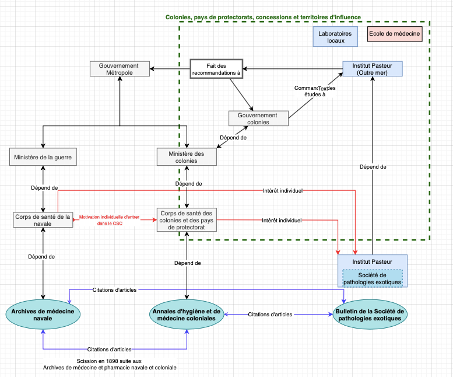
\includegraphics[width=10cm]{./images/schema-AHMC-AMN-BSPE}
    \caption{Schéma des relations entretenues entre les trois revues}
    \label{Schema-BDD-memoire}
\end{figure}




\begin{figure}
    \centering
    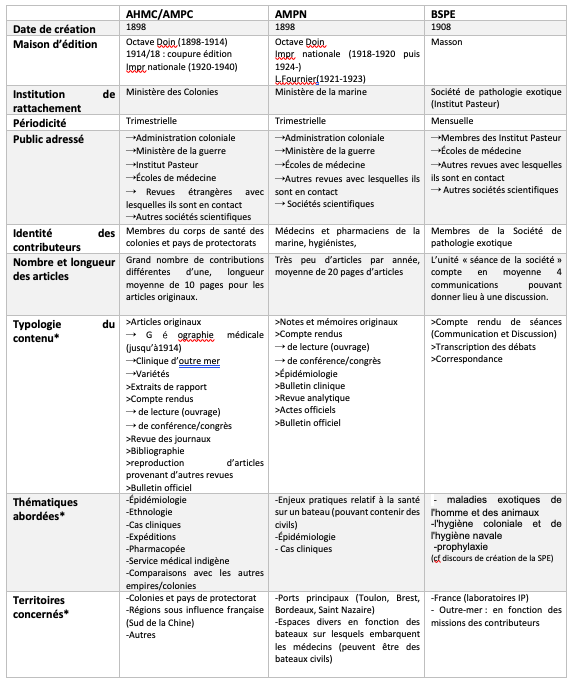
\includegraphics[width=10cm]{./images/Tableau comparaison}
    \caption{Tableau explicatif de chacune des revues}
    \label{Schema-BDD-memoire}
\end{figure}



\end{document}
